%%%%%%%%%%%%%%%%%%%%%%%%%% ch2-part1
\begin{frame}[shrink]
\frametitle{ch2.信号检测与估计理论的基础知识}
\framesubtitle{概率论简单回顾}
\tableofcontents[hideallsubsections]
\end{frame}


\section{样本空间,事件域,概率}

\begin{frame}{随机现象}
随机现象:\\
~\\
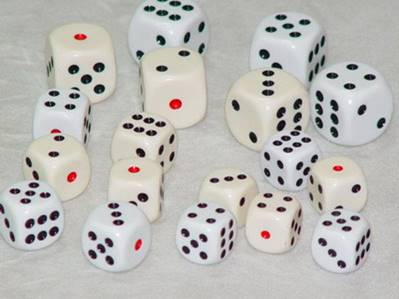
\includegraphics[scale=0.5]{die1}
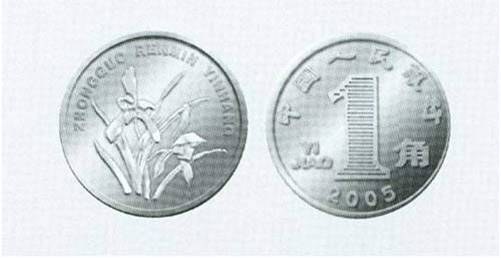
\includegraphics[scale=0.5]{coin1}\\
落叶的运动轨迹,气泡的扩散,灯泡的寿命
\begin{block}{随机现象特点}
	\begin{itemize}
		\item 至少两种可能
		\item 不确定性
	\end{itemize}
\end{block}
\end{frame}

\begin{frame}{概率论中的三个组成部分}
\begin{itemize}
	\item 样本空间$\Omega$
	\item 事件域$\mathcal{F}$
	\item 概率$P$
\end{itemize}
\end{frame}

\begin{frame}
\begin{itemize}
	\item \textbf{样本空间$\Omega$}:一个随机试验所有可能出现的结果的全体,称为随机事件的样本空间。\\
	每一个可能的结果称为基本事件,它们的全体就是样本空间。
	\item \textbf{样本点$\xi_k$}:随机试验的一个结果,就是某个基本事件,也就是$\Omega$中的一个元素。\\
	$\Omega=\{\xi_k|k=1,\dots,n\}$
	\item \textbf{随机事件$A$}: 样本空间中的某个子集称为随机事件,简称事件(事件是集合)。
    \item \textbf{事件域$\mathcal{F}$}: 样本空间中的某些子集构成的满足如下条件的集合,称为事件域(又称$\sigma^-$域)。
	\begin{itemize}
		\item[(1)] $\Omega\in\mathcal{F}$
		\item[(2)] 若$A\in\mathcal{F}$, 则$A$的补$\overline{A}\in\mathcal{F}$
		\item[(3)] 若$A_n\in\mathcal{F}, n=1,2,\dots$, 则$\bigcap\limits_{n=1}^{\infty}A_n\in\mathcal{F}$
	\end{itemize}
\end{itemize}
\end{frame}

\begin{frame}
\begin{example}
	一个盒子中有10个相同的球,5个 白色,5个黑色,搅匀后从中任意摸取一球。\\
	~\\
	样本点: $\xi_1=\{\text{取得白球} \}$, $\xi_2=\{\text{取得黑球} \}$\\
	样本空间: $\Omega=\{\xi_1,\xi_2\}$
\end{example}
\begin{example}
	一个盒子中有10个相同的球,编号1,2,...,10, 从中取一球。\\
	样本空间: $\Omega=\{1,2,\dots,10\}$\\
	随机事件: $A=\{\text{6号球} \}=\{6\}$, $B=\{\text{偶数编号球} \}=\{2,4,6,8,10\}$, $\overline{B}=\{\text{奇数编号球}\}$,$C=\{\text{编号小于等于5的球} \}=\{1,2,3,4,5\}$\\
	事件A是基本事件,而B和C则由多个基本事件所组成,并且$A,B,C\subset\Omega$。
\end{example}
\textit{空集$\emptyset$可以看作$\Omega$的子集,在任意一次试验中不可能有此事件发生,称为不可能事件。}
\end{frame}

\begin{frame}{事件$A$的概率$P(A)$}
  事件域中的元素就是随机事件。如果这些事件的随机性能够由定义在事件域$\mathcal{F}$上的具有非负性,归一性和可列加性的实函数$P(A)$来确定,则称$P$是定义在二元组$(\Omega,\mathcal{F})$上的概率,而称$P(A)$为事件$A$的概率。
  \begin{enumerate}
  	\item[(1)] 非负性。 $P(A)\ge 0$
  	\item[(2)] 归一性。 $P(\Omega)=1$
    \item[(3)] 可列加性。$A_1,A_2,...,A_n$互不相容$(A_i\cap A_j=\emptyset,i\ne j)$,则$P(A_1\cup A_2\cup\dots\cup A_n) = P(A_1)+P(A_2)+\cdots+P(A_n)$
  \end{enumerate}
\end{frame}

\begin{frame}
\frametitle{等可能概型(古典概型)}
\begin{itemize}
	\item 样本空间的元素(即基本事件)只有有限个,不妨设为$n$个,$\Omega=\{\xi_1,\xi_2,\dots,\xi_n\}$
	\item 每个基本事件出现的可能性是相等的,即有$P(\xi_1)=P(\xi_2)=\cdots=P(\xi_n)$
	\item 事件域$\mathcal{F}$为$\Omega$的所有子集的全体,即是$Pwr(\Omega),\Omega$的幂集,共有$2^n$个事件,$\emptyset\in\mathcal{F},\Omega\in\mathcal{F}$。
	\item 由概率的有限可加性知\\
	$1=P(\Omega)=\sum\limits_{i=1}^{n}P(\xi_i)\implies P(\xi_i)=\frac{1}{n},(i=1,\dots,n)$
	\item 对任意一个随机事件$A\subseteq\mathcal{F}$, 如果$A$是$k$个基本事件的和,即$A=\{\xi_{i_1}\}\cup \{\xi_{i_2}\}\cup\cdots\cup\{\xi_{i_k}\}$, 则
	$$P(A)=\frac{k}{n}=\frac{\text{$A$中所包含的基本事件数}}{\text{基本事件总数}}$$
\end{itemize}
\end{frame}

\begin{frame}
\begin{example}
	将一枚硬币抛掷3次,(1) 设事件$A_1$为``恰有一次出现正面'', 求$P(A_1)$;
	(2) 设事件$A_2$为``至少一次出现正面'',求$P(A_2)$。
	\begin{enumerate}
		\item 正面用$H$表示, 反面用$T$表示。则\\
		样本空间$\Omega=\{HHH,HHT,HTH,HTT,THH,THT,TTH,TTT\}$\\
		事件$A_1=\{HTT,THT,TTH\}$。\\
		$\Omega$中包含有限个元素, 且由对称性知, 每个基本事件发生的可能性相同。所以, $P(A_1)=\frac{3}{8}$。
		\item 由于$\overline{A_2}=\{TTT\}$, 于是\\
		$P(A_2)=1-P(\overline{A_2})=1-\frac{1}{8}=\frac{7}{8}$
	\end{enumerate}
\end{example}
\end{frame}

\begin{frame}
\frametitle{样本空间的选取}
为求一个事件的概率,样本空间可以有不同的取法,但一定要保证基本事件和求概事件数的计算都要在\textbf{同一个样本空间}中进行,否则会导致谬误!
\begin{example}
	一个盒子中有10个相同的球,编号1,2,...,10, 从中取一球,求此球的号码为偶数的概率。\\
	样本空间$\Omega=\{1,2,\dots,10\}$\\
	事件$A=\{\text{偶数编号球} \}=\{2\}\cup\{4\}\cup\{6\}\cup\{8\}\cup\{10\}=\{2,4,6,8,10\}$。\\
	$P(A)=\frac{|A|}{n}=\frac{5}{10}=\frac{1}{2}$
\end{example}
另外一种解法:$\Omega=\{A,\overline{A}\},A=\{\text{编号为偶数的球}\},\overline{A}=\{\text{编号为奇数的球}\},\mathcal{F}=\{\emptyset,\Omega,A,\overline{A}\}$,由$A,\overline{A}$的对称性,即得$P(A)=\frac{1}{2}$

\end{frame}

\begin{frame}
\frametitle{样本空间的选取}
\begin{block}{Notes}
	\begin{itemize}
		\item 两种解法的样本空间$\Omega$不同(从而事件域$\mathcal{F}$是不同的)。
		\begin{enumerate}
			\item $\Omega=\{1,2,\dots,10\}$ 
			\item $\Omega=\{A,\overline{A}\}$
		\end{enumerate}
	   \item 严格地说,两者所描述的随机试验是不同的。\\
	   例如对于第二种解法来说,$B=\{\text{号码为4的球}\}$并不属于事件域$\mathcal{F}$,就是说$B$不是一个事件,从而也就没有概率可言。\\
	   但对第一种解法,$B$是事件,而且$P(B)=\frac{1}{10}$。
	   \item 一定要保证基本事件和求概事件数的计算都要在\textbf{同一个样本空间}中进行。
	\end{itemize}
\end{block}
\end{frame}

\section{条件概率,全概率公式}

\begin{frame}{条件概率}
\begin{definition}
	若$\Omega,\mathcal{F},P$是一个概率空间,$B\in\mathcal{F}$, 且$P(B)>0$,则对任意的$A\in\mathcal{F}$,称
	$$P(A|B)=\frac{P(AB)}{P(B)}$$
	为在已知事件B发生的条件下,事件A发生的条件概率。
\end{definition}

\begin{columns}%0.6 0.4表示相对比例
	\column{0.4\textwidth}%<1->
\[P(A|B)=\frac{S_{AB}}{S_B}=\frac{S_{AB}/S_\omega}{S_B/S_\omega}=\frac{P(AB)}{P(B)} \]
	\column{0.4\textwidth}%<1->
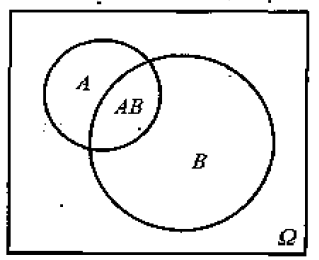
\includegraphics[scale=0.2]{P(AB)}
\end{columns}
\end{frame}

\begin{frame}{条件概率的性质及其推论}
\begin{block}{条件概率$P(\bullet|B)$的具备概率的三个基本性质}
	\begin{enumerate}
		\item 非负性: 对任意的$A\in F, P(A|B)\ge 0$;
		\item 规范性: $P(\Omega|B)=1$;
		\item 可列加性: 对任意的一列两两互不相容的事件$A_i(i=1,2,\dots)$, 有
		\[P\left[\bigcup\limits_{i=1}^{+\infty}(A_i|B)\right]=\sum\limits_{i=1}^{+\infty}P(A_i|B) \]
	\end{enumerate}
\end{block}
\begin{corollary}
概率的乘法公式:  $P(AB)=P(B)P(A|B)$
\end{corollary}

\begin{corollary}
	$P(A_1A_2\cdots A_n)=P(A_1)P(A_2|A_1)P(A_3|A_1A_2)\cdots P(A_n|A_1A_2\cdots A_{n-1})$
\end{corollary}
\end{frame}

\begin{frame}
\begin{example}
	一个家庭中有两个小孩,已知其中有一个是女孩,问这时另一个小孩也是女孩的概率有多大?
	
	\medskip
	$\Omega=$\{(男,男),(男,女),(女,男),(女,女)\}\\
	$A=$\{已知有一个是女孩\}=\{(男,女),(女,男),(女,女)\}\\
	$B=$\{另一个也是女孩\}=\{(女,女)\}\\
	于是所求概率为\\
	$P(B|A)=\frac{P(AB)}{P(A)}=\frac{1/4}{3/4}=\frac{1}{3}$
\end{example}
\end{frame}

\begin{frame}{概率树/全概率公式}
概率树思想:为了求解复杂事件的概率,往往可以先把它分解成两个(或若干个)互不相容的较简单的事件之并。求出这些较简单事件的概率,再利用加法公式即得所要求的复杂事件的概率。把这个方法一般化,便的到下述定理。
\begin{theorem}
	设$B_1,B_2,\cdots$是一列互不相容的事件,且有
	\[\bigcup_{i=1}^{+\infty}B_i=\Omega,P(B_i)>0 \]
	则对任一事件A,有
	\[P(A)=\sum_{i=1}^{+\infty}P(B_i)P(A|B_i) \]	
\end{theorem}
\end{frame}

\begin{frame}
\begin{example}
	某工厂有4条流水线生产同一种产品, 该4条流水线的产品分别占总产量的15\%, 20\%, 30\%, 35\%, 又这4条流水线的不合格品率依次为0.05, 0.04, 0.03及0.02. 现从出厂产品中任取一件, 问
	\begin{enumerate}
		\item 恰好抽到不合格品的概率为多少? 
		\item 第4条流水线应承担的责任?
	\end{enumerate} 
\end{example}
\end{frame}

\begin{frame}[shrink]
解: (1) 令
\begin{align*}
A&=\{\text{任取一件,恰好抽到不合格品} \}\\
B&=\{\text{任取一件,恰好抽到第$i$条流水线的产品}, (i=1,2,3,4) \}
\end{align*}
于是由全概率公式可得
\begin{align*}
P(A)&=\sum\limits_{i=1}^4P(B_i)P(A|B_i)=0.15\times 0.05+0.20\times 0.04+0.30\times 0.03+0.35\times 0.02\\
&=0.0315=3.15\%
\end{align*}
实际上,$P(A|B_i)$可以从过去生产的产品中统计出来,称为\textbf{先验概率}。\\
(2) 从概率论的角度考虑可以按$P(A|B_i)$的大小来追究第$i$条$i=1,2,3,4$流水线的责任。\\
$P(AB_4)=P(B_4)P(A|B_4)=0.35\times 0.02=0.007$\\
由条件概率的定义知
\begin{align*}
P(B_4|A)=\frac{P(AB_4)}{P(A)}=\frac{P(B_4)P(A|B_4)}{\sum\limits_{i=1}^4P(B_i)P(A|B_i)}=\frac{0.007}{0.0315}\approx 0.222
\end{align*}
\end{frame}

\begin{frame}{相互独立事件}
条件概率: $P(B|A)=\frac{P(AB)}{P(A)}$\\
一般的概率乘法公式: $P(AB)=P(A)P(B|A)$\\
如果``事件B发生与否不受事件A的影响'': $P(B)=P(B|A)$\\
乘法公式变为: $P(AB)=P(A)P(B)$
\begin{definition}
对任意的两个事件A,B,若
\[P(AB)=P(A)P(B)\]
成立,则称事件A,B是相互独立的,简称为独立的。	
\end{definition}
\begin{block}{依这个定义,不难验证:}
	若A与B相互独立,则$\{\emptyset,A,\overline{A},\Omega\}$中的任意一个与$\{\emptyset,B,\overline{B},\Omega\}$中的任意一个仍相互独立。
\end{block}
\end{frame}

\begin{frame}[shrink]
		分别掷两枚均匀的硬币,令
		\begin{align*}
		A=\{\text{硬币甲出现正面} \}\quad	B=\{\text{硬币乙出现正面} \}
		\end{align*}
		验证事件$A,B$是相互独立的。
 \begin{proof}
			$$\text{样本空间}=\{\text{(正,正),(正,反),(反,正),(反,反)}\} $$
			共还有4个基本事件,它们是等可能的,各有概率为1/4,而
			\begin{align*}
			A&=\{\text{(正,正),(正, 反)}\} \\
			B&=\{\text{(正,正),(反, 正)}\} \\
			AB&=\{\text{正,正}\}
			\end{align*}
			由此知 \[P(A)=P(B)=\frac{1}{2}\]
			这时有 \[P(AB)=\frac{1}{4}=P(A)P(B)\]
			成立,所以A, B事件是相互独立的。
 \end{proof}
\end{frame}

\section{随机变量}

\begin{frame}
\begin{definition}
	设$(\Omega,\mathcal{F},P)$是一概率空间,$X=X(\xi),\xi\in\Omega$是定义在$\Omega$上的单值实函数,如果对任一实数$x$, 集合$\{\xi|X(\xi)\le x\}\in\mathcal{F}$ 则称$X=X(\xi)$为$(\Omega,\mathcal{F},P)$上的一个\textbf{随机变量}。
	
	随机变量$X(\xi)$的定义域为样本空间$\Omega$,它的值域是实数R。所以,随机变量$X(\xi)$实际上是一个映射,这个映射为每个来自概率空间的结果(样本点)$\xi$赋予一个实数$x$。这种映射必须满足条件:
	\begin{itemize}
		\item[(1)] 对任一$x$,集合$\{\xi|X(\xi)\le x\}\in\mathcal{F}$(即,使得$X(\xi)\le x$的所有样本点$\xi$所组成的集合)是这个概率空间中的一个事件,并有确定的概率$P\{X(\xi)\le x\}$;
		\item[(2)] $P\{X(\xi)=\infty \}=0$, $P\{X(\xi)=-\infty \}=0$
	\end{itemize}
\end{definition}
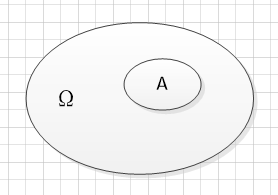
\includegraphics[scale=0.2]{geometry}
\end{frame}

\begin{frame}
\begin{example}
	将一枚硬币抛掷3次,正面用$H$表示, 反面用$T$表示, 则样本空间
	\[\Omega=\{HHH,HHT,HTH,HTT,THH,THT,TTH,TTT\} \]
	令随机变量$X(\xi)$表示投掷得到正面的总数。则
	\[ 
		X=X(\xi)=
		\begin{cases}
		3, &\xi=\{HHH\}\\
		2, &\xi=\{HHT,HTH,THH\}\\
		1, &\xi=\{HTT,THT,TTH\}\\
		0, &\xi=\{TTT\}
		\end{cases}
	\]
	$X=2$, 对应样本点的集合$A=\{HHT,HTH,THH\}$,是一个事件, 其概率$P\{X=2\}=P(A)=3/8$。类似地有
	\[ P\{X\le 1\}=P\{\{X=0\}\cup\{X=1\}\}=P\{HTT,THT,TTH,TTT\}=\frac{1}{2} \]
\end{example}
\end{frame}

\begin{frame}
随机变量的取值随试验的结果而定, 而试验的各个结果出现有一定的概率, 因而随机变量的取值有一定的概率。
\begin{definition}
	设$X=X(\xi)$是随机变量, 若$L$是一个实数集合, $L\subseteq\mathbb{R}, $将$X$在$L$上取值写成$\{X\in L\}$. 它表示事件$B=\{\xi|X(\xi)\in L \}$. 即$B$是由$\Omega$中使得$X(\xi)\in L$的所有样本点$\{\xi\}$所组成的事件, 此时有
    \[P\{X\in L\}=P(B)=P\{\xi|X(\xi)\in L\} \]
\end{definition}
\begin{block}{Notes}
	随机变量$X=X(\xi)$就是试验结果(即样本点)和实数之间的一一对应关系。虽然在试验之前不能肯定随机变量$X=X(\xi)$会取哪一个数值,但是对于任一实数$a$, 我们可以研究$\{X=X(\xi)=a \}$发生的概率, 也就是$X(\xi)$取值的统计规律。
\end{block}
\end{frame}

\begin{frame}{随机变量的分布函数}
\begin{definition}
	设$X$是随机变量, 对$\forall x\in\mathbb{R}$, 称函数
	\[F(x)=P\{X\le x\}, -\infty<x<\infty\]
	为随机变量$X$的一维(累积)分布函数[(cumulative) distribution function]。
\end{definition}
对于任意实数$x_1,x_2(x_1<x_2)$,有
\[P\{x_1<X\le x_2\}=P\{X\le x_2\}-P\{X\le x_1\}=F(x_2)-F(x_1) \]
\begin{block}{Notes}
	如果将$X$看成是数轴上的随机点的坐标, 那么, 分布函数$F(x)$在$x$处的函数值就表示$X$落在区间$(-\infty,x]$上的概率。
\end{block}
\end{frame}

\begin{frame}
\begin{block}{分布函数性质}
	\begin{enumerate}
		\item 单调不减性: 对$\forall x_1<x_2$, 恒有$F(x_1)\le F(x_2)$\\
		对于任意实数$x_1,x_2(x_1<x_2)$,有
		\[F(x_2)-F(x_1)=P\{x_1<X\le x_2\}\ge 0 \]
		\item 规范性: $0\le F(x)\le 1$, 且
		\[ F(-\infty)=\lim\limits_{x\to -\infty}F(x)=0,\quad F(+\infty)=\lim\limits_{x\to +\infty}F(x)=1 \]
		\item 右连续性: 对$\forall x_0$, 恒有$F(x_0+0)=\lim\limits_{x\to x_0^+}F(x)=F(x_0)$
	\end{enumerate}
\end{block}
\begin{block}{几何说明}
	将$X\in [0,x]$的端点$x$沿数轴无限向左移动(即$x\to -\infty$), 则``随机点$X$落在点$x$左边''这一事件趋于不可能事件, 从而概率趋于$0$, 即有$F(-\infty)=0$;
	
	\medskip
	将$X\in [0,x]$的端点$x$沿数轴无限向右移动(即$x\to \infty$), 则``随机点$X$落在点$x$左边''这一事件趋于必然事件, 从而概率趋于$1$, 即有$F(\infty)=1$;
\end{block}

\end{frame}

\begin{frame}{随机变量的概率密度函数$p(x)$}
\begin{definition}
	设连续随机变量$X$的\textbf{一维累积分布函数}为$F(x)$, 如果$F(x)$对$x$的一阶导数存在,则有
	\[p(x)\mathop{=}^{def}\frac{dF(x)}{dx}\]
	式中, $p(x)$称为随机变量$X=X(\xi)$的\textbf{一维概率密度函数}, 简称概率密度函数(probability density function, p.d.f)
\end{definition}
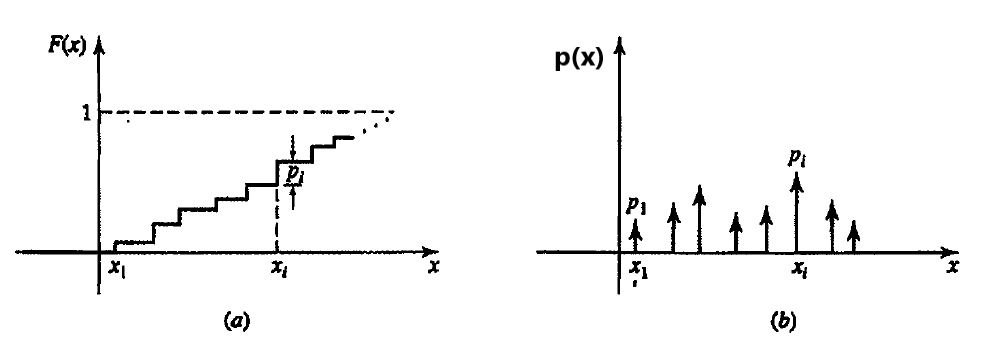
\includegraphics[scale=0.4]{pi}
\end{frame}

\begin{frame}[shrink]
\frametitle{随机变量概率密度函数$p(x)$的性质}
\begin{enumerate}
	\item 根据随机变量$x(\xi)$的$p(x)$与$F(x)$的关系, 有
	\[F(x)=\int_{-\infty}^{x}p(u)du\]
	\item 对所有$x$, p(x)是非负函数,即
	\[p(x)\ge 0,\quad -\infty<x<+\infty \]
	\item $p(x)$对$x$的全域积分结果等于1, 一般表示为
	\[\int_{-\infty}^{\infty}p(x)dx=1\]
	\item 随机变量$x(\xi)$落在区间$[x_1,x_2]$内的概率为
	\[P\{x_1\le x(\xi)\le x_2\}=F(x_2)-F(x_1)=\int_{x_1}^{x_2}p(x)dx\]
\end{enumerate}
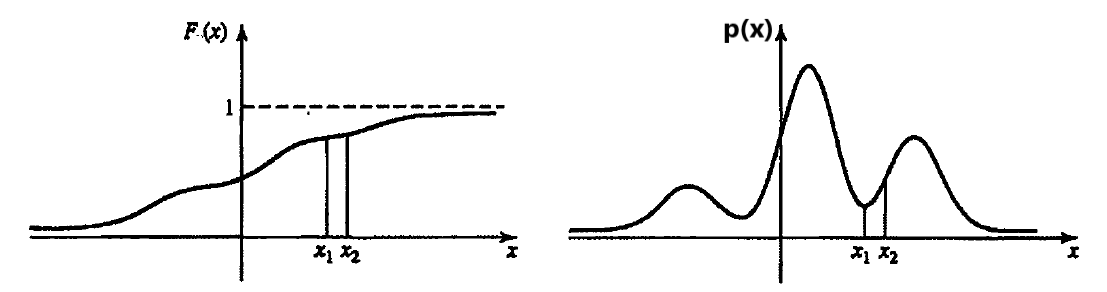
\includegraphics[scale=0.3]{Fx-px2}
\end{frame}

\section{离散型随机变量及其分布律}

\begin{frame}[shrink]
%\frametitle{离散型随机变量}
\begin{definition}[离散型随机变量]
	定义在样本空间$\Omega$上,取值于实数域$\mathbb{R}$,且只取\textcolor{blue}{有限个或可列个值}的变量$X=X(\xi)$, 称作是\textbf{一维(实值)离散型随机变量}。\\
\end{definition}

\begin{definition}[离散型随机变量的概率]
	设离散型随机变量$X$所有可能取的值为$x_k(k=1,2,\dots)$, $X$取各个可能值的概率, 即事件$\{X=x_k\}$的概率为
	\[P\{X=x_k\}=p_k, k=1,2,\dots\]
\end{definition}

由概率的定义, $p_k$满足如下两个条件: 
\begin{enumerate}
	\item $p_k\ge 0, k=1,2,\dots$
	\item $\sum\limits_{k=1}^{\infty}p_k=1$\\
	因为$\{X=x_1\}\cup\{X=x_2\}\cup\cdots$是必然事件, 且$\{X=x_j\}\cap\{X=x_k\}=\emptyset, k\ne j$故
	\[1=P[\bigcup_{k=1}^{\infty}\{X=x_k\}]=\sum_{k=1}^{\infty}P\{X=x_k\}=1 \]
\end{enumerate}
\end{frame}

\begin{frame}{离散型随机变量$X$的分布律}
离散型随机变量$X$的分布律的解析表达式:
	\[P\{X=x_k\}=p_k, k=1,2,\dots\]
可用表格形式表示如下:
\begin{block}{离散型随机变量$X$的分布律}
	%\begin{tabular}{c|c|c|c|c|c|}
	\begin{tabular}{c|ccccc}
		%\hline 
		$X$ & $x_1$ & $x_2$ & $\cdots$ & $x_n$ & $\cdots$\\ 
		\hline 
		$p_k$ & $p_1$ & $p_2$ & $\cdots$ & $p_n$ & $\cdots$\\ 
		%\hline 
	\end{tabular} 
\end{block}

\begin{example}
	某产品40件,其中次品3件,现从中任取3件。(1) 求取出的3件产品中所含次品数$X$的分布律; (2) 求取出的产品中至少有一件次品的概率; (3) 求离散型随机变量$X$的分布函数$F(x)$。
\end{example}
\end{frame}

\begin{frame}
\begin{block}{解:}
(1) \begin{tabular}{ll}
	$P\{X=0\}=\frac{C_{37}^{3}}{C_{40}^{3}}=0.7865$ & $P\{X=1\}=\frac{C_{3}^{1}C_{37}^{2}}{C_{40}^{3}}=0.2022$ \\ 
	$P\{X=2\}=\frac{C_{3}^{2}C_{37}^{1}}{C_{40}^{3}}=0.0112$ & $P\{X=3\}=\frac{C_{3}^{3}}{C_{40}^{3}}=0.0001$ \\ 
\end{tabular}\\ 
(2) \quad $P\{X\ge 1\}=1-P\{X=0\}=1-0.7865=0.2135$\\
(3) 由分布函数定义得:
$F(x)=P\{X\le x\} =
\begin{cases}
0,      & x<0 \\
0.7865, & 0\le x<1 \\
0.9887, & 1\le x<2 \\
0.9999, & 2\le x<3 \\
1,      & x\ge 3
\end{cases} $
\end{block}
\begin{columns}%0.6 0.4表示相对比例
	\column{0.4\textwidth}%<1->
	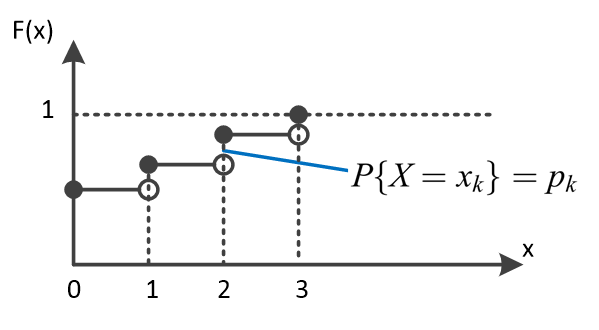
\includegraphics[scale=0.22]{fx}
	\column{0.6\textwidth}%<1->
	由$F(x)$的图示看到, $F(x)$是一个阶梯状的右连续函数($F(x+0)=F(x)$),在$x=k$处有跳跃,跃度为在$X=k$处的概率$p_k=P\{X=k\}$。	
\end{columns}
\end{frame}

\begin{frame}
\begin{columns}
\column{0.4\textwidth}
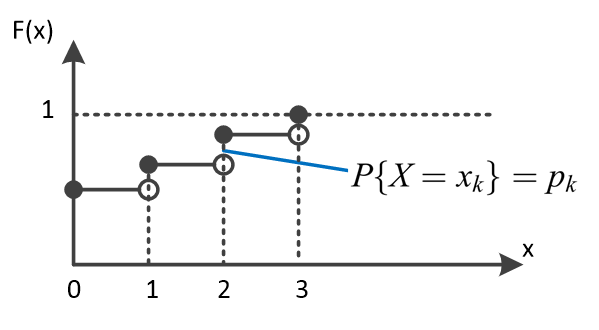
\includegraphics[scale=0.22]{fx}
\column{0.6\textwidth}
由随机变量$X$的分布函数$F(x)$, 可以计算
\begin{block}{}
\begin{align*}
P(X \le x) &= F(x)\\
P(X = x) &= F(x)-F(x-0) \\
P(X < x) &= F(x-0) \\
P(X > x) &= 1- F(x) \\
P(X \ge x) &= 1-F(x-0)
\end{align*}
进一步,形如$\{x_1\le X\le x_2\},\{x_1< X< x_2\},\{x_1< X\le x_2\}, \{x_1\le X< x_2\}$等一些事件及它们经过有限次或可列次并、交、差运算以后的概率,都可以由$F(x)$计算出来。
\end{block}
\end{columns}
\begin{block}{}
\textcolor{blue}{$F(x)$全面地描述了随机变量$X$的统计规律。}
\end{block}
\end{frame}

\section{狄拉克函数(Dirac函数/$\delta$函数)}

\begin{frame}{狄拉克函数(Dirac函数/$\delta$---函数)}
\begin{definition}[$\delta$---函数]
	对于任意的无穷次可微的函数$f(t)$, 如果满足:
	$$\int_{-\infty}^{\infty}\delta (t)f(t)dt=\lim\limits_{\varepsilon\to 0}\int_{-\infty}^{\infty}\delta_{\varepsilon}(t)f(t)dt $$
	其中:
	\[
	\delta_{\varepsilon}(t)=\begin{cases}
	0,&t<0\\
	\frac{1}{\varepsilon}, & 0\ge t<\varepsilon\\
	0, &t>\varepsilon
	\end{cases}
	\]
	则称$\delta_\varepsilon(t)$的弱极限为$\delta$函数,记为$\delta(t)$
	显然, 对于任意的$\varepsilon>0$, 有:
	$$\int_{-\infty}^{\infty}\delta_{\varepsilon}(t)dt=\int_{-\infty}^\infty\frac{1}{\varepsilon}dt=1\implies \int_{-\infty}^\infty\delta(t)dt=1$$
\end{definition}
\end{frame}

\begin{frame}{狄拉克函数(Dirac函数/$\delta$---函数)}
\begin{block}{注}
\begin{enumerate}
	\item $\delta(t)$在$t=0$点的取值为$\infty$, 在$t\ne 0$点的取值为0, 并且满足$\int_{-\infty}^{\infty}\delta(t)dt=1$。
	\item 工程(信号处理等)上$\delta$---函数也称为单位脉冲或单位冲激函数。
\end{enumerate}
\end{block}
\begin{block}{$\delta$---函数的筛选性质}
若$f(t)$为无穷此可微的函数,则有:$\int_{I}\delta(t)f(t)dt=f(0) $\\
其中$I$是包含点$t=0$的任意区间。特殊地, 有:$\int_{-\infty}^{\infty}\delta(t)f(t)dt=f(0) $\\
更一般地,我们有:
$$\int_{-\infty}^{\infty}\delta(t-t_0)f(t)dt=f(t_0) $$
\end{block}
\end{frame}

\begin{frame}[shrink]
\frametitle{离散型随机变量分布律的$\delta$---函数表示}
设离散型随机变量$X$的分布律为: $P\{X=x_i\}=p_i,i=1,2,\dots$, 则由$\delta$---函数的筛选性质可以定义离散型随机变量$X$的概率密度函数为:
$$p(x)=\sum\limits_{i=0}^{\infty}p_i\delta(x-x_i)$$
因为,由$\delta$---函数的筛选性质,离散型随机变量$X$的分布函数可以表示为:
$$F(x)=P\{X\le x\}=\sum\limits_{x_i\le x}p_i=\int_{-\infty}^{x}\sum\limits_{i=1}^{\infty}p_i\delta(u-x_i)du$$
\[P\{X=x_i\}=F(x_i)-F(x_i^{-})=p_i\]
\begin{columns}
	\column{0.4\textwidth}
	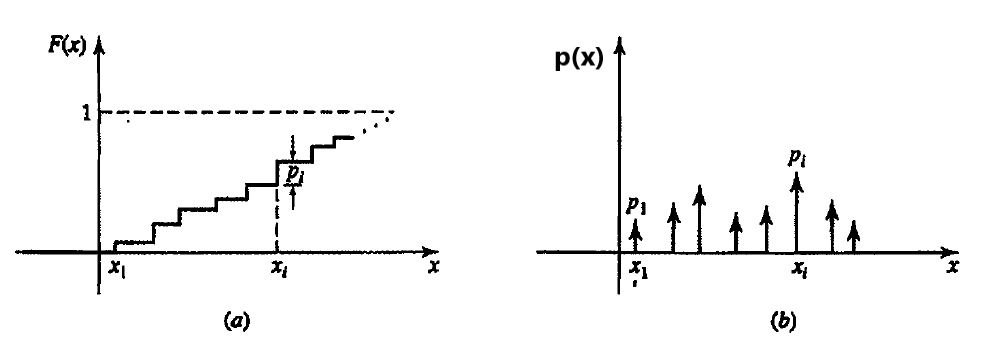
\includegraphics[scale=0.2]{pi}
	\column{0.4\textwidth}
	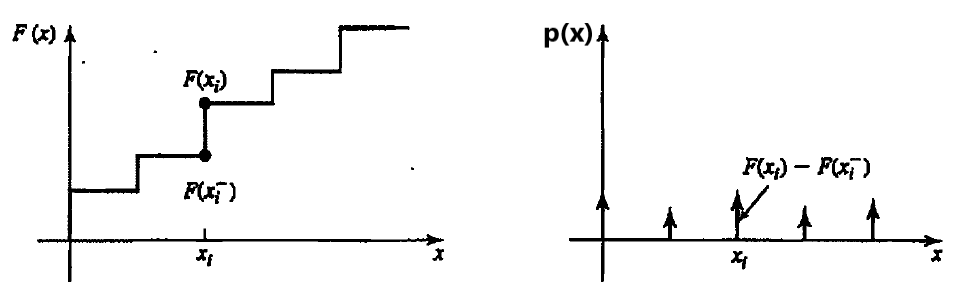
\includegraphics[scale=0.2]{Fx-px}
\end{columns}
\end{frame}

\begin{frame}[shrink]
\frametitle{离散型随机变量与连续性随机变量的统一}
\begin{block}{}
	工程上,常用离散型随机变量分布律的$\delta$---函数表示法,将离散型随机变量的分布律表示成概率密度函数的形式,因此与连续型随机变量的概率密度函数$p(x)$一样进行统一处理。
\end{block}
$$P\{x_1\le X\le x_2\}=\int_{x_1}^{x_2}p(x)dx$$
离散型随机变量:
	$$F(x)=P\{X\le x\}=\sum\limits_{x_i\le x}p_i=\int_{-\infty}^{x}\sum\limits_{i=1}^{\infty}p_i\delta(u-x_i)du$$
	$$p(x)=\sum\limits_{i=0}^{\infty}p_i\delta(x-x_i)$$
连续型随机变量:
	$$p(x)\mathop{=}^{def}\frac{dF(x)}{dx},\quad F(x)=P\{X\le x\}=\int_{-\infty}^{x}p(u)du$$

\end{frame}

\begin{frame}[shrink]
\begin{example}
抛掷一枚硬币: 样本空间: $\Omega=\{H,T\}$, $H$表示正面, $T$表示反面。正面的概率$p$, 反面的概率$q$. 定义随机变量$X=X(\xi),\xi\in \Omega$满足:
	\[X(\xi=H)=1\qquad X(\xi=T)=0,\]
	求分布函数$F(x)$和概率密度函数$p(x)$,其中: $-\infty<x<\infty$.
\end{example}
\begin{align*}
&P\{X=0\}=q,\quad P\{X=1\}=p\\
&F(x)=P\{X\le x\}=\sum\limits_{x_i\le x}p_i=\int_{-\infty}^{x}\sum\limits_{i=1}^{\infty}p_i\delta(u-x_i)du\\
&p(x)=\sum\limits_{i=0}^{\infty}p_i\delta(x-x_i)
\end{align*}
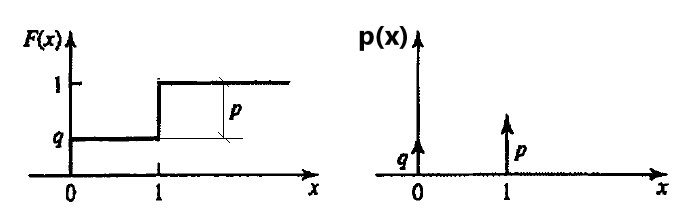
\includegraphics[scale=0.4]{coin-tossing} 
X\end{frame}

\begin{frame}[shrink]
\begin{example}
事件A, 试验的样本空间: $\Omega=\{A,\overline{A},\emptyset \}$. 定义随机变量$X=X(\xi)$,
满足:
\begin{align*}
	X(\xi)=1, &\quad \xi\in A\\
	X(\xi)=0, &\quad \xi\in\overline{A}
\end{align*}
\end{example}
\begin{align*}
&P\{X=1\}=P(A)=p,\quad P\{X=0\}=P(\overline{A})=q=1-p\\
&F(x)=P\{X\le x\}=\sum\limits_{x_i\le x}p_i=\int_{-\infty}^{x}\sum\limits_{i=1}^{\infty}p_i\delta(u-x_i)du\\
&p(x)=\sum\limits_{i=0}^{\infty}p_i\delta(x-x_i)
\end{align*}
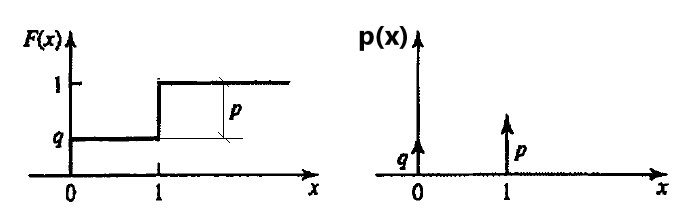
\includegraphics[scale=0.4]{coin-tossing}
\end{frame}

\begin{frame}[shrink]
\begin{example}
抛掷两枚硬币: 随机变量$X=X(\xi)$表示正面数目。\\
样本空间: $\Omega=\{HH,HT,TH,TT\}$, $H$表示正面, $T$表示反面。\\
随机变量$X(HH)=2,\quad X(HT)=1, \quad X(TH)=1, \quad X(TT)=0$ \\
求$F(x)$和$p(x)$.
\end{example}
\begin{align*}
&P\{X=0\}=\frac{1}{4}, \quad P\{X=1\}=\frac{2}{4},\quad P\{X=2\}=\frac{1}{4}\\
&F(x)=P\{X\le x\}=\sum\limits_{x_i\le x}p_i=\int_{-\infty}^{x}\sum\limits_{i=1}^{\infty}p_i\delta(u-x_i)du\\
&p(x)=\sum\limits_{i=0}^{\infty}p_i\delta(x-x_i)
\end{align*}
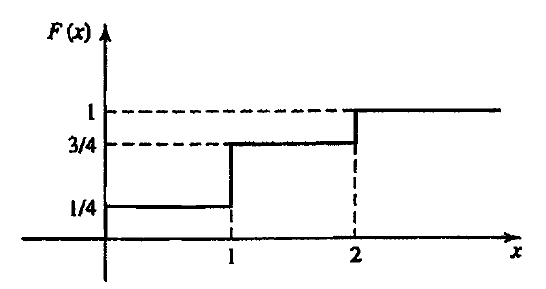
\includegraphics[scale=0.3]{coin-tossing2} \medspace \medspace
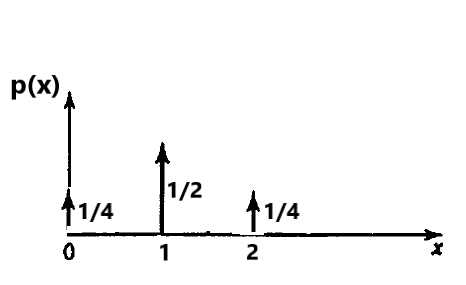
\includegraphics[scale=0.3]{coin-tossing22}
\end{frame}

\begin{frame}[shrink]
掷一枚骰子: 样本空间: $\Omega=\{f_1,f_2,f_3,f_4,f_5,f_6\}$。定义随机变量$X=X(\xi),\xi\in \Omega$满足:$X(f_i)=10i$
求$F(x)$和$p(x)$,其中: $-\infty<x<\infty$.\\
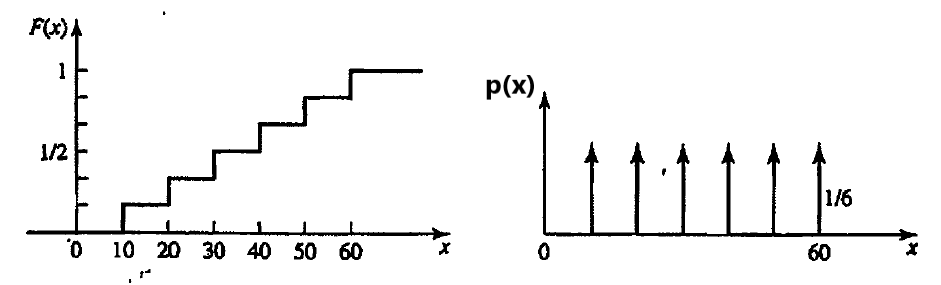
\includegraphics[scale=0.4]{die}
\begin{align*}
F(100)&=P\{X(\xi)\ge 60 \}=P(\Omega)=1\\
F(35)&=P\{X(\xi)\le 35 \}=P\{f_1,f_2,f_3 \}=\frac{3}{6} \\
F(30.01)&=P\{X(\xi)\le 30.01 \}=P\{f_1,f_2,f_3 \}=\frac{3}{6} \\
F(30)&=P\{X(\xi)\le 30 \}=P\{f_1,f_2,f_3 \}=\frac{3}{6} \\
F(29.9)&=P\{X(\xi)\le 29.9 \}=P\{f_1,f_2 \}=\frac{2}{6} \\
\end{align*}
\end{frame}



